\documentclass[diploma]{BMSTU-IU8}

\student{И. И. Иванов}
\theme{Создание отчёта \\ по НИРС \\ или ВКР}
\group{ИУ8-999}

\supervisor{П. П. Петров}
\researchConsultant{П. П. Петров}
\designConsultant{П. П. Петров}
\technologicalConsultant{П. П. Петров}
\economicsConsultant{П. П. Петров}
\lawsConsultant{П. П. Петров}
\normController{П. П. Петров}

% \theme{Тест \hfill} % Тема для НИРСа заполняется по-другому
\studentFullName{Иванов Иван Иванович}
\profile{10У101}
\speciality{10.05.01 <<Компьютерная безопасность>>}
\specialization{10.05.01\_01 <<Математические методы защиты информации>>}
\supervisorWithDegree{доцент, к.т.н. Иванов И. И.}

% \newacronym{bd}{БД}{База данных.}
\newacronym{subd}{СУБД}{Система управления базами данных.}
\newacronym{ddl}{DDL}{Data Definition Language.}
\newacronym{dql}{DQL}{Data Query Language.}
\newacronym{dml}{DML}{Data Manipulation Language.}
\newacronym{dcl}{DCL}{Data Control Language.}
\newacronym{lsn}{LSN}{Log sequence number.}
\newacronym{id}{ID}{Identifier.}
\newacronym{uuid}{UUID}{Universally unique identifier.}


\newglossaryentry{id1}{
    name={База данных (БД)},
    description={это организованная коллекция данных, которая структурирована таким образом, чтобы данные можно было легко хранить, управлять, изменять и извлекать.},
}

\newglossaryentry{id7}{
    name={Бакет},
    description={это логический контейнер, в который помещаются данные для
    распределения по шардам (физическим серверам или узлам). Это абстракция,
    которая связывает ключ шардирования с конкретным шардом.}
}

\newglossaryentry{id6}{
    name={Кластер},
    description={это совокупность нескольких репликасетов, каждый из которых чаще всего хранит разный набор данных.}
}

\newglossaryentry{id11}{
    name={Ребалансировка},
    description={процесс перевозки бакетов с одного шарда на другой.}
}

\newglossaryentry{id5}{
    name={Репликасет (replicaset, набор реплик, шард)},
    description={это группа узлов, работающих в режиме репликации и объединенных для обеспечения отказоустойчивости и доступности данных.}
}

\newglossaryentry{id2}{
    name={Система управления базами данных (СУБД)},
    description={это программное обеспечение, предназначенное для создания, управления и обеспечения доступа к базам данных. Оно позволяет пользователям определять, создавать, изменять и управлять базой данных, а также обеспечивает взаимодействие между пользователями и базой данных через запросы и команды. Основные функции включают хранение, поиск, обновление и удаление данных, а также обеспечение целостности, безопасности и управления доступом к данным.}
}

\newglossaryentry{id4}{
    name={Спейс (space)},
    description={это основная логическая единица хранения данных Tarantool, аналогичная таблице в традиционных реляционных базах данных. Спейс содержит набор записей, каждая из которых называется кортежем (tuple). Структура спейса определяется схемой, которая включает количество и типы полей в кортежах, а также индексы для быстрого доступа к данным.}
}

\newglossaryentry{id10}{
    name={Шардирование},
    description={это принцип проектирования базы данных, при котором данные
    разбиваются на части и размещаются на разных наборах реплик (репликасеты,
    шарды).}
}

\newglossaryentry{id8}{
    name={LSN},
    description={это монотонно возрастающий идентификатор записи.}
}

\newglossaryentry{id9}{
    name={Vclock},
    description={это массив LSN, идентификаторами в котором являются ID узлов. Vclock представляет собой набор логических счетчиков для каждого узла в кластере, позволяя определить, какие изменения были применены на конкретном узле и какие еще предстоит синхронизировать.}
}

\addbibresource{main.bib}

\begin{document}
    % \maketitle
    \setcounter{page}{3} % Устанавливает счётчик страниц

    \structure{РЕФЕРАТ}

Алгоритм Шора серьёзно поставил под вопрос безопасность информации, основанную
на криптосистемах с открытым ключом. Однако для взлома широко используемой
схемы RSA-2048 требуются миллионы физических кубитов, что значительно превышает
текущие технические возможности. Здесь мы сообщаем об универсальном квантовом
алгоритме факторизации целых чисел, объединяющем классическую редукцию базиса
решетки с квантовым алгоритмом приближённой оптимизации (QAOA). Количество
требуемых кубитов равно $O(\log N / \log\log N)$, что сублинейно относительно
битовой длины целого числа $N$, делая этот алгоритм самым экономичным по числу
кубитов алгоритмом факторизации на сегодняшний день. Мы экспериментально
демонстрируем алгоритм, факторизуя целые числа размером до 48 бит с помощью 10
сверхпроводящих кубитов, что является наибольшим целым числом, факторизованным
на квантовом устройстве. Мы оцениваем, что квантовая схема с 372 физическими
кубитами и глубиной в тысячи операций необходима для того, чтобы бросить вызов
RSA-2048 при помощи нашего алгоритма. Наше исследование демонстрирует
значительные перспективы для ускорения применения текущих шумных квантовых
компьютеров и прокладывает путь к факторизации больших целых чисел, имеющих
реальное криптографическое значение.
 % Реферат

    \tableofcontents % Содержание
    \termsanddefenitions % Термины и определения
    % \listofabbreviations % Перечень сокращений и обозначений

    \structure{ВВЕДЕНИЕ}

Квантовые вычисления вступили в эпоху шумных квантовых устройств промежуточного
масштаба (NISQ) \cite{cite_1, cite_2}. Важной задачей эпохи NISQ является
демонстрация того, что устройства NISQ могут превзойти классические компьютеры
при решении задач с практической значимостью, то есть достижение практического
квантового преимущества. Алгоритмы, требующие минимальных ресурсов и
использующие ограниченное число доступных кубитов и глубину схем для решения
задач, сложных для классических вычислений, имеют особую важность. Вариационные
квантовые алгоритмы, использующие гибридную схему вычислений
«классика+квантовые вычисления», обладают значительным потенциалом для
получения значимого квантового преимущества в эпоху NISQ \cite{cite_3, cite_4,
cite_2, cite_5, cite_6}. Одним из таких алгоритмов является квантовый алгоритм
приближённой оптимизации (QAOA) \cite{cite_5}, первоначально предложенный для
решения задач на собственные значения, который впоследствии широко применялся в
различных областях, таких как химическое моделирование \cite{cite_7, cite_8},
машинное обучение \cite{cite_9}, а также инженерные приложения \cite{cite_10,
cite_11}.

Факторизация целых чисел является одной из важнейших основ современной
информационной безопасности \cite{cite_12}. Экспоненциальное ускорение
факторизации алгоритмом Шора \cite{cite_13} является выдающимся примером
превосходства квантовых вычислений. Однако выполнение алгоритма Шора на
отказоустойчивом квантовом компьютере требует значительных ресурсов
\cite{cite_14, cite_15}. На сегодняшний день наибольшее целое число,
факторизованное алгоритмом Шора на существующих квантовых системах, это число
21 \cite{cite_16, cite_17, cite_18}. Альтернативно, факторизация целых чисел
может быть сведена к задаче оптимизации, решаемой посредством адиабатических
квантовых вычислений (AQC) \cite{cite_19, cite_20, cite_21, cite_22} или QAOA
\cite{cite_23}. Более крупные числа были факторизованы этими методами на
различных физических системах \cite{cite_24, cite_25, cite_26, cite_27}.
Максимальные числа, факторизованные на данный момент, включают 291311 (19 бит)
в системе NMR \cite{cite_26}, 249919 (18 бит) на квантовом отжигателе D-Wave
\cite{cite_25}, 1099551473989 (41 бит) на сверхпроводящем устройстве
\cite{cite_27}. Однако следует отметить, что некоторые из факторизованных чисел
были специально подобраны с особыми структурами \cite{cite_28}, поэтому
наибольшее число, факторизованное универсальным методом на реальной физической
системе, на сегодняшний день составляет 249919 (18 бит).

В данной работе мы предлагаем универсальный квантовый алгоритм факторизации
целых чисел, требующий лишь сублинейные квантовые ресурсы. Алгоритм основан на
классическом алгоритме Шнорра \cite{cite_29, cite_30}, использующем редукцию
базиса решётки для факторизации целых чисел. Мы используем QAOA для оптимизации
наиболее трудоёмкой части алгоритма Шнорра, что ускоряет общее время
факторизации. Для целого числа $N$, имеющего $m$ бит, количество требуемых
кубитов в нашем алгоритме составляет $O(m / \log m)$, что сублинейно
относительно битовой длины числа $N$. Это делает наш алгоритм наиболее
экономным по числу кубитов по сравнению с существующими алгоритмами, включая
алгоритм Шора. С использованием данного алгоритма нами успешно факторизованы
числа 1961 (11 бит), 48567227 (26 бит) и 261980999226229 (48 бит) с
использованием, соответственно, 3, 5 и 10 кубитов на сверхпроводящем квантовом
процессоре. Число в 48 бит (261980999226229) также является наибольшим целым
числом, факторизованным универсальным методом на реальном квантовом устройстве.
Далее мы оцениваем квантовые ресурсы, необходимые для факторизации RSA-2048.
Согласно нашим расчётам, квантовая схема с 372 физическими кубитами и глубиной
порядка тысяч операций необходима для факторизации RSA-2048 даже в самой
простой одномерной системе. Подобный масштаб квантовых ресурсов, вероятно,
станет достижимым на устройствах NISQ в ближайшем будущем.

 % Введение

    \structure{ОСНОВНАЯ~ЧАСТЬ}

\section{Характеристика организации}

ВK Цифровые Технологии – подразделение VK, развивающее продукты и сервисы для
цифрового бизнеса. В основе экосистемы решений VK Цифровые технологии лежит
многолетний опыт развития интернет-сервисов и технологии на базе открытого
кода. VK Цифровые Технологии предоставляет готовые сервисы для решения бизнес
задач любой сложности, занимается заказной разработкой и управлением
ИТ-инфраструктурой на аутсорсе \cite{VkTech}.

В портфеле VK цифровые Технологии — облачные сервисы VK Cloud Solutions,
платформа in-memory вычислений Tarantool, платформа взаимодействия бизнеса и
государства VK Tax Monitoring, а также линейка программных продуктов для
управления персоналом, автоматизации производства и бизнес-процессов.

Tarantool как продукт появился 4 апреля 2016 года, когда Mail.ru Group (на
данный момент известная как VK) сообщила о создании нового направления бизнеса,
в рамках которого компания начала предоставлять корпоративным клиентам услуги в
области хранения данных.

Изначально Tarantool применялся только в собственных проектах Mail.ru, в том
числе в почтовом сервисе и облачном хранилище «Облако Mail.Ru». Затем компания
превратила эту СУБД в продукт с открытым исходным кодом, который к началу
апреля 2016 года внедрен рядом российских и международных компаний. В
частности, Tarantool начал использоваться сервисом бесплатных объявлений Avito,
социальной сетью знакомств Badoo и разработчиком систем информационной
безопасности Wallarm.

На сегодняшний день Tarantool активно используется в банковской сфере (среди
клиентов Tarantool можно выделить ВТБ, Альфа Банк, Банк Открытие и Газпромбанк)
и для ретейла и e-commerce (Магнит, Wildberries, Ситилинк, X5Group)
\cite{Tarantool}.

    \include{contents/2-01-tarantool-replication}
    \section{Файловый JOIN}

Одним из требований заказчика является возможность продолжения подключения реплики (JOIN) к репликасету с места остановки в случае сбоя. Эта функциональность будет обеспечиваться так называемым файловым JOIN, подробности которого описаны в данной части. Он работает только для анонимных реплик, что достаточно для CDC.

Такое требование вызвано большим временем выкачивания read-view во время стадии initial JOIN, в течение которого могут происходить многочисленные ошибки сети. Однако продолжить скачивание после переподключения нельзя, так как read-view нигде не сохраняется.

Вместо read-view было принято решение использовать файлы snapshot для отсылки изначального состояния. Это делается с помощью модификации протокола запроса IPROTO\_FETCH\_SNAPSHOT, который отныне выглядит следующим образом:

\begin{enumerate}
    \item Реплика посылает запрос IPROTO\_FETCH\_SNAPSHOT, указывая IPROTO\_CURSOR (описание см. ниже).
    \item Мастер отвечает на IPROTO\_FETCH\_SNAPSHOT vclock-ом снапшота, который он собирается посылать.
    \item После чего следует пересылка данных, каждая запись которых промаркирована с помощью LSN.
    \item В случае обрыва подключения, реплика посылает VCLOCK, полученный в пункте б, и LSN, до которого она успела получить данные.
\end{enumerate}

Так как vclock и данные с LSN уже посылались и до этого, именяется только IPROTO\_FETCH\_SNAPSHOT, приведенный на рисунке ~\ref{fig:fig04}.

\begin{figure}
  \centering
  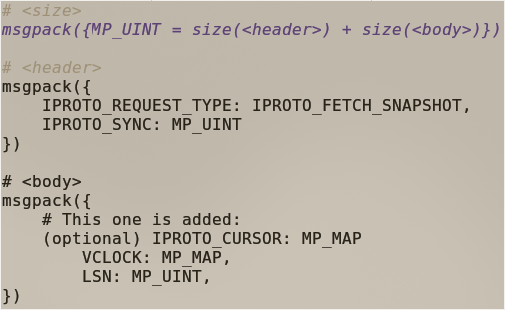
\includegraphics[scale=2.00]{inc/listing.png}
  \caption{Изменения в запросе IPROTO\_FETCH\_SNAPSOT}
  \label{fig:fig04}
\end{figure}

Добавляется новое поле в тело запроса: IPROTO\_CURSOR, представляющее собой таблицу с полями VCLOCK и LSN. Она указывает, откуда необходимо продолжить скачивание файла. Она может иметь следующие значения:

\begin{itemize}
    \item \textit{\{nil, nil\}} - используется скачивания read-view для обратной совместимости
    \item \textit{\{\{0\}, 0\}} - курсор неизвестен, мастер берет последний сделанный snapshot и посылает его.
    \item \textit{\{VCLOCK, LSN\}} - курсор известен реплике и она хочет продолжить скачивание. Находим snapshot, идентифицируемый vlock-ом и начинаем пересылку с определенного LSN.
\end{itemize}

Мастер при получении IPROTO\_CURSOR проверяет, что снапшот с запрашиваемым vclock-ом еще существует и что в нем есть запрашиваемый LSN. В противном случае реплике возвращается ошибка, она должна снова передать \textit{\{\{0\}, 0\}} и начать скачивание уже другого снапшота заново.

    \section{Персистентный GC}

Следующим требованием заказчика было сохранение данных для анонимных реплик. Эта функциональность будет обеспечиваться персистентным GC, описание которого приводится в данной части.

Это требование вытекает из того факта, что репликация идет только из xlog файлов. Мастер постоянно отслеживает, кому и какие xlog файлы нужны в репликасете, и не удаляет их. Однако для анонимных реплик это не делается, так как они не входят в репликасет. Когда xlog файлы, которые еще не были среплицированы на анонимную реплику, удаляются, то реплика вынуждена делать процесс ребутстрапа, включающий в себя выкачивание состояния БД с нуля. Это приводит к существенному понижению доступности анонимной реплики.

Было принято решение полностью переделать систему GC, так как до этого состояние GC находилось в памяти и после перезапуска узел не знал, какие файлы нужно сохранять, а какие можно удалять. Это приводило к тому, что узел был вынужден ждать подключения всех реплик к текущему узлу.

\textbf{Локальный спейс \_gc\_consumers}

Теперь состояние GC сохраняется в новом локальном спейсе \_gc\_consumers, который имеет следующий формат, приведенный в таблице~\ref{tab:tab1}.

\begin{table}
    \centering
    \caption{Формат \_gc\_consumers}
    \begin{tabular}{|r|c|l|}\hline
        Поле & Имя & uuid \\ \hhline{~--}
             & Тип & string \\ \hline
        Поле & Имя & vclock \\ \hhline{~--}
             & Тип & map    \\ \hline
    \end{tabular}
    \label{tab:tab1}
\end{table}

UUID используется вместо id реплики, так как отныне xlog файлы могут также сохраняться для анонимных реплик, у которых id равно 0. Объединение всех анонимных реплик в одну строку не является оптимальным решением.

Для каждой из реплик создается GC consumer, который отслеживает, до какого vclock реплика уже получила данные. Их реализация (в памяти) остается без изменений, однако теперь они создаются\/удаляются с использованием on\_replace триггера спейса \_gc\_consumers. Во время запуска узла они будут созданы автоматически.

\textbf{Подключение обычных реплик}

Для обычных реплик появляется новый on\_replace триггер на спейс \_cluster, в который реплика вставляется после окончания фазы initial JOIN. Этот тригер вставляет кортеж в спейс \_gc\_consumers, что вызовет создание GC consumer для данной реплики. Удаление реплики из спейса \_cluster вызывает удаление записи из \_gc\_consumers. Прямое удаление реплики из \_gc\_consumers запрещено.

Таким образом, процесс подключение неанонимной реплики выглядит следующим образом:

\begin{enumerate}
    \item Реплика хочет быть присоединенной к репликасету и отправляет IPROTO\_JOIN.
    \item Мастер создает read-view, посылает его реплике. Реплика вставляется в спейс \_cluster, on\_replace триггер создает запись в \_gc\_consumers. Отныне файлы сохраняются для этой реплики.
    \item Реплика входит в фазу FOLLOW.
\end{enumerate}

\textbf{Подключение анонимных реплик}

Так как анонимная реплика нигде не сохраняется, как это делается для обычных реплик (\_cluster), нам необходимо добавить новый флаг в IPROTO\_FETCH\_SNAPSHOT: IPROTO\_IS\_PERSISTENT\_GC. По умолчанию флаг равен false, GC consumer-ы для анонимных реплик не создаются. Также этот флаг необходимо добавить в IPROTO\_SUBSCRIBE (инициация фазы FOLLOW).

Таким образом, процесс подключения анонимной реплики выглядит следующим образом:

\begin{enumerate}
    \item Реплика отправляет IPROTO\_FETCH\_SNAPSHOT с флагом IPROTO\_IS\_PERSISTENT\_GC. Реплика получает в ответ read-view или файл. Отныне xlog файлы хранятся для нее.
    \item Реплика отправляет IPROTO\_SUBSCRIBE с тем же флагом.
\end{enumerate}

Однако мы не можем позволить таким GC consumer-ам существовать вечно, как это сделано для обычных реплик. Иначе место на диске может быть быстро израсходовано. А потому добавляется новая опция конфигурирования: wal\_anon\_gc\_timeout. Она показывает, сколько секунд живет GC consumer, после момента, когда мы в последний раз общались с репликой.

    \section{Фильтрация репликационного потока}

Поcледним требованием заказчика была фильтрация репликационного потока. Это требование вытекает из необходимости снижения нагрузки на CDC реплики и заключается в частичной пересылки данных мастером.

Основные моменты:

\begin{itemize}
    \item Фильтрация репликации производится по именам спейсов. Фильтруется как процесс подключения реплик, так и процесс применения изменений. Клиент может подписаться на изменения спейсов, которые еще не были созданы.
    \item Запрошенные спейсы реплицируются вместе с их метаданным: \_space, \_index, \_truncate частично реплицируются, только данные, относящиеся к запрошенным спейсам, будут отправлены.
    \item При изменении имени или удаление спейса клиент получает информацию об этом последней записью. Последующие изменения (в случае переименования) не посылаются. Если будет создан спейс с именем, который запрошен клиентом, то клиент начинает получать данные из него.
\end{itemize}

Для обеспечения фильтрации в IPROTO\_FETCH\_SNAPSHOT и IPROTO\_SUBSCRIBE добавляется новая опция: IPROTO\_SPACE\_NAME\_FILTER, представляющая собой массив названий необходимых спейсов. Если опция не указана, полная репликация используется для обратной совместимости.

Управление подпиской на фильтрованный репликационный поток:

\begin{itemize}
    \item Добавление нового еще не существующего спейса к фильтру. Клиент может инициировать IPROTO\_SUBSCRIBE в любой момент, чтобы добавить новый спейс.
    \item Удаление спейса из фильтра. Делается таким же образом.
    \item Добавление уже существующего спейса в фильтр. Недопустимое изменение фильтра. На момент изменения фильтра клиент уже имеет какой-то vclock и мы продолжим посылать данные с этого vclock-a. Однако метаданные спейса будут скорее всего пропущены, так как спейс уже был создан до изменения фильтра.
\end{itemize}


    \conclusion

В ходе прохождения практики был проведён комплексный анализ механизма
шардирования в СУБД Tarantool. Основное внимание было уделено изучению
архитектуры модуля \texttt{vshard}, принципов распределения данных и
обеспечения согласованности при выполнении операций в шардированном кластере.

Были рассмотрены и проанализированы существующие подходы к реализации
Map-Reduce запросов по репликам. В результате исследования выявлены ключевые
проблемы, связанные с обеспечением консистентности данных при выполнении
распределённых запросов, и предложена альтернативная реализация.

Практическая значимость работы заключается в:
\begin{itemize}
    \item Систематизации знаний о работе шардированного кластера Tarantool;
    \item Выявлении ограничений существующей реализации модуля \texttt{vshard};
    \item Разработке предложений по расширению функциональности для поддержки
        Map-Reduce операций по репликам.
\end{itemize}

Полученные результаты могут быть использованы для дальнейшего развития модуля
шардирования Tarantool и улучшения его безопасности. Проведённое исследование
демонстрирует важность комплексного подхода к проектированию распределённых
систем и необходимость тщательного анализа требований к согласованности данных.

Результаты работы подтверждают возможность реализации эффективного механизма
выполнения Map-Reduce запросов по репликам в шардированной среде с соблюдением
требований к консистентности данных и производительности системы.


    \printbibliography
\end{document}
